\chapter{Appendix}

\begin{figure}[hbt!]
    \centering
    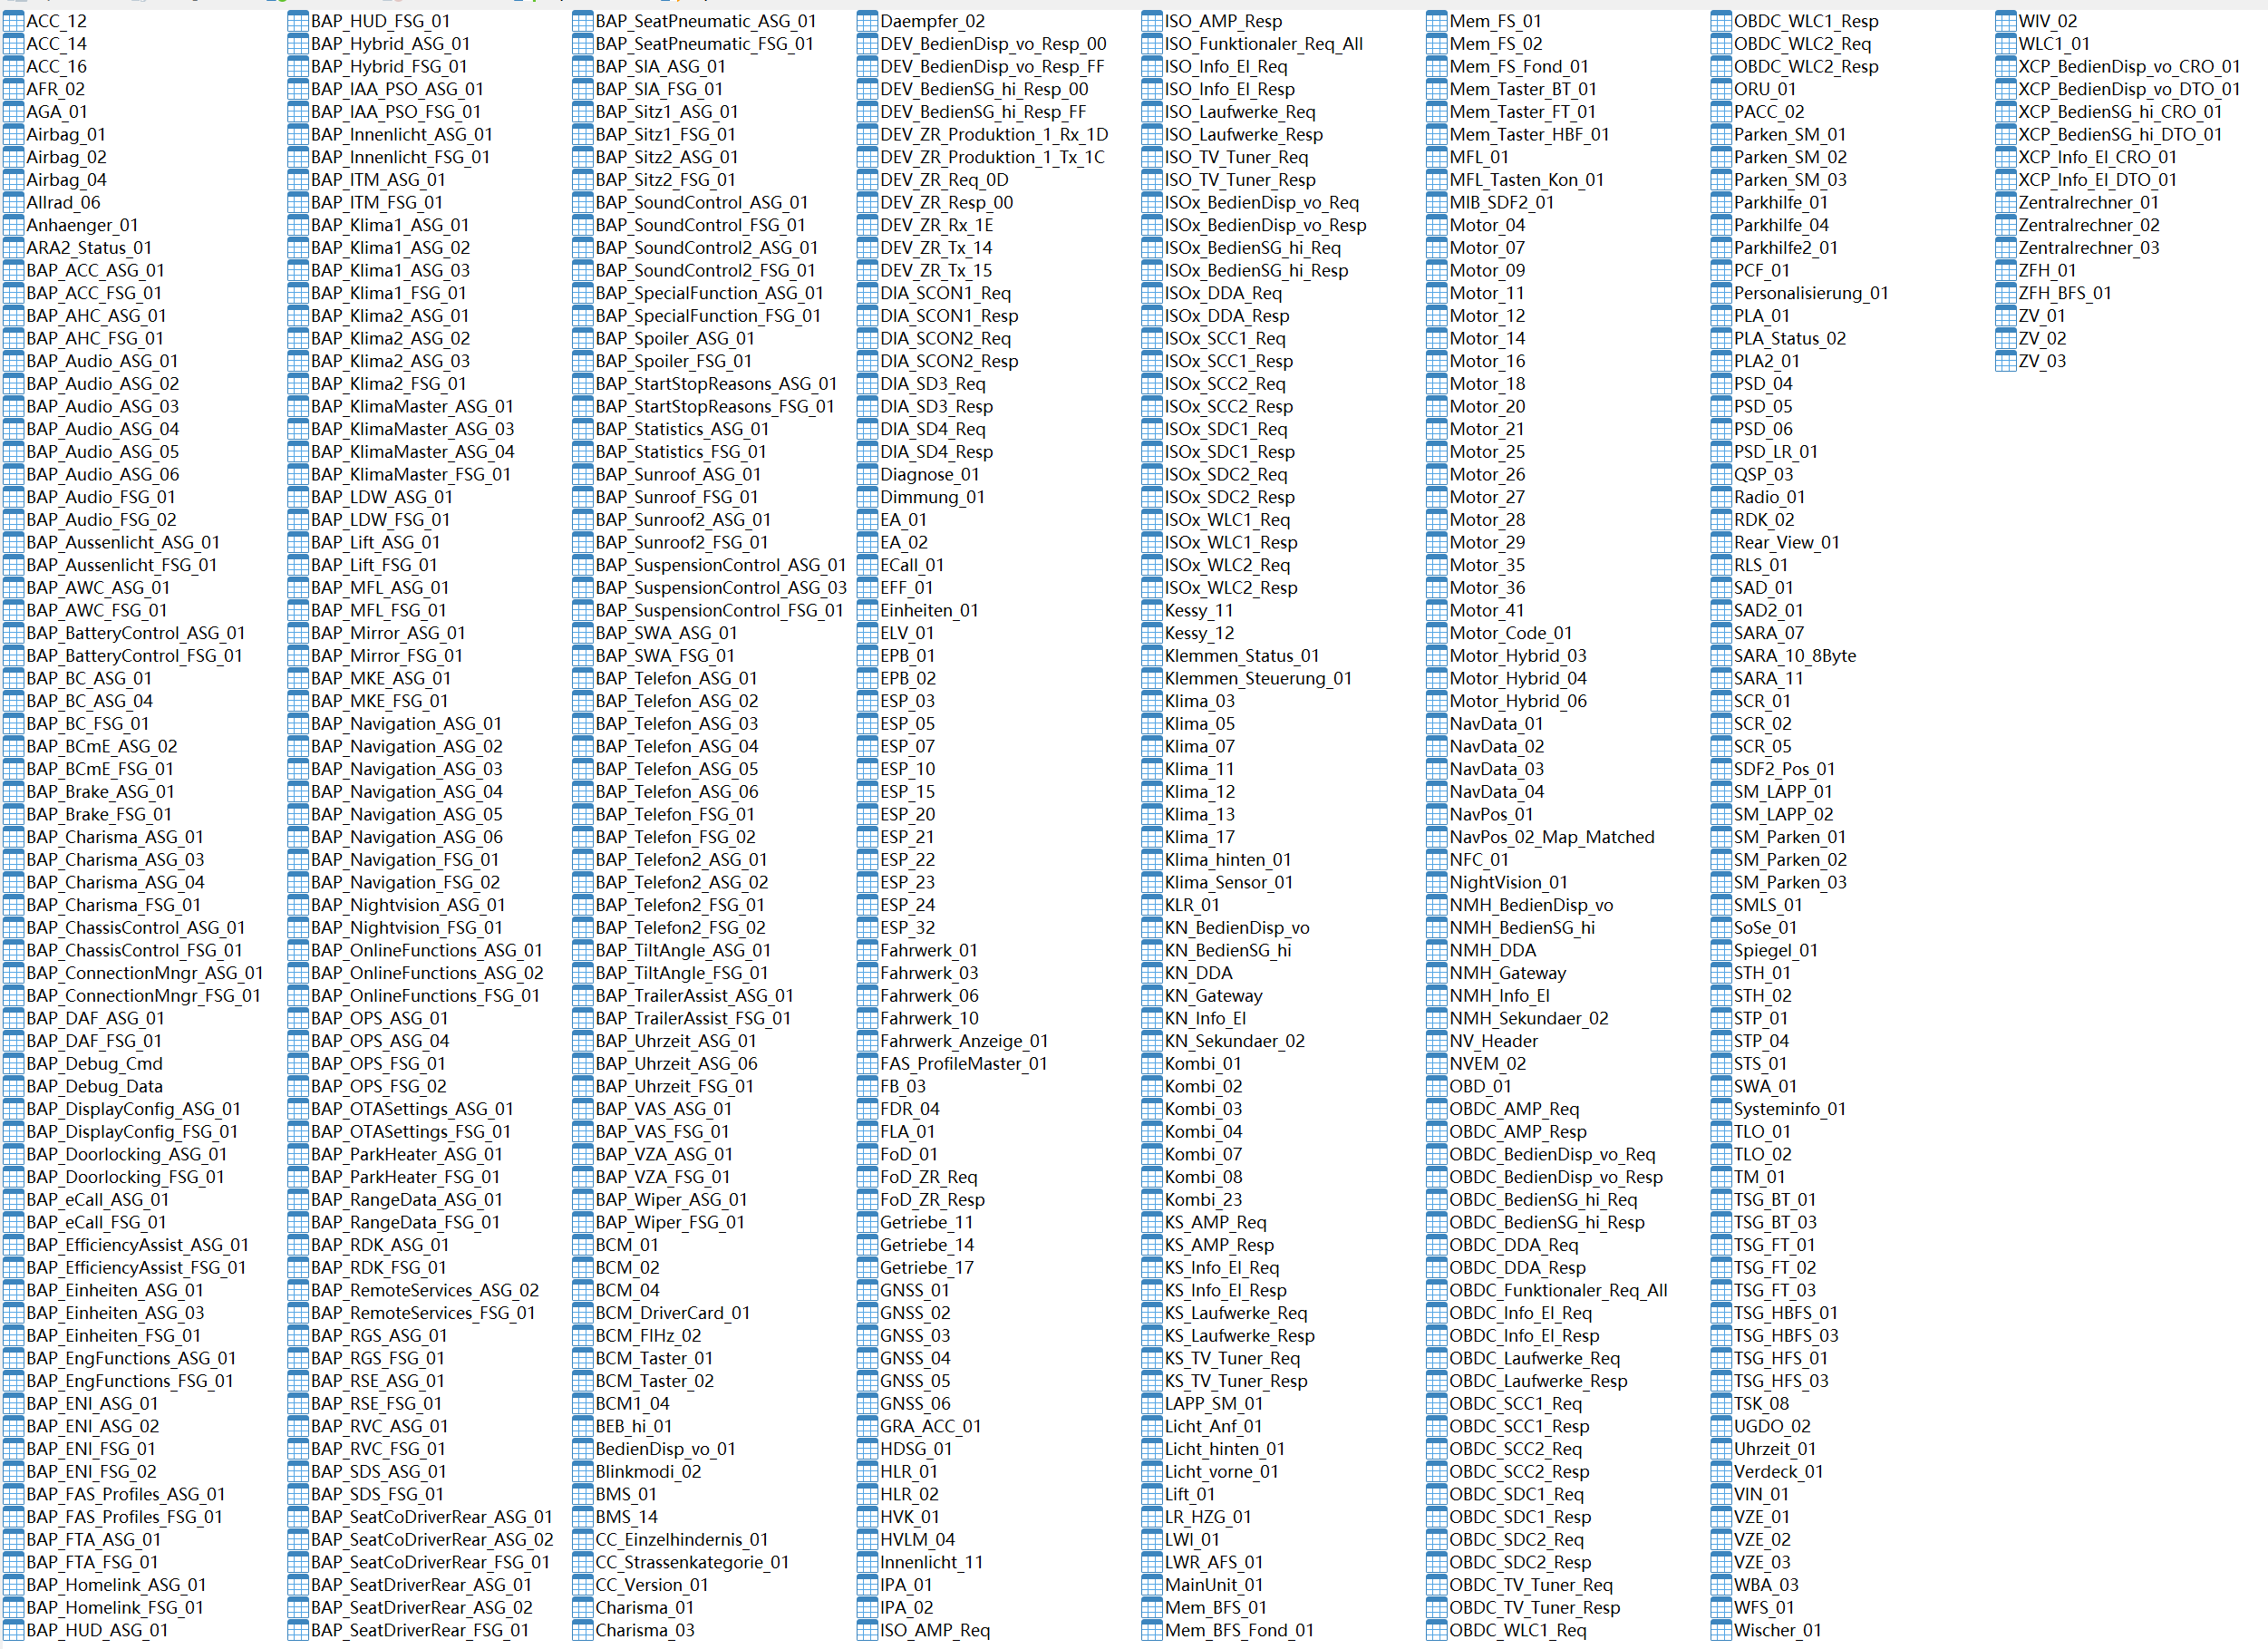
\includegraphics[width=1.0\textwidth]{gfx/DBC_table.png}
    \caption{CAN-ID}
    \label{fig:can_idtable}
\end{figure}

\begin{minted}[
frame=lines,
framesep=2mm,
baselinestretch=1.2,
bgcolor=LightGray,
fontsize=\footnotesize,
linenos
]{bash}
# Aggregate query of MySQL 
SELECT COUNT(*) FROM audi_a8.Motor_12 WHERE ts BETWEEN ${time_start} AND ${time_end}
SELECT AVG(MO_Drehzahl_01) FROM audi_a8.Motor_12 WHERE ts BETWEEN ${time_start} AND ${time_end}
SELECT SUM(MO_Drehzahl_01) FROM audi_a8.Motor_12 WHERE ts BETWEEN ${time_start} AND ${time_end}
SELECT MAX(MO_Drehzahl_01) FROM audi_a8.Motor_12 WHERE ts BETWEEN ${time_start} AND ${time_end}
SELECT MIN(MO_Drehzahl_01) FROM audi_a8.Motor_12 WHERE ts BETWEEN ${time_start} AND ${time_end}

# Aggregate query of ClickHouse
SELECT COUNT(*) FROM audi_a8.Motor_12 WHERE ts BETWEEN ${time_start} AND ${time_end}
SELECT AVG(MO_Drehzahl_01) FROM audi_a8.Motor_12 WHERE ts BETWEEN ${time_start} AND ${time_end}
SELECT SUM(MO_Drehzahl_01) FROM audi_a8.Motor_12 WHERE ts BETWEEN ${time_start} AND ${time_end}
SELECT MAX(MO_Drehzahl_01) FROM audi_a8.Motor_12 WHERE ts BETWEEN ${time_start} AND ${time_end}
SELECT MIN(MO_Drehzahl_01) FROM audi_a8.Motor_12 WHERE ts BETWEEN ${time_start} AND ${time_end}

# Aggregate query of Cassandra
SELECT COUNT(*) FROM audi_a8.Motor_12 WHERE ts BETWEEN ${time_start} AND ${time_end}
SELECT AVG(MO_Drehzahl_01) FROM audi_a8.Motor_12 WHERE ts BETWEEN ${time_start} AND ${time_end}
SELECT SUM(MO_Drehzahl_01) FROM audi_a8.Motor_12 WHERE ts BETWEEN ${time_start} AND ${time_end}
SELECT MAX(MO_Drehzahl_01) FROM audi_a8.Motor_12 WHERE ts BETWEEN ${time_start} AND ${time_end}
SELECT MIN(MO_Drehzahl_01) FROM audi_a8.Motor_12 WHERE ts BETWEEN ${time_start} AND ${time_end}

# Aggregate query of InfluxDB
use audi_a8;
SELECT COUNT(MO_Drehzahl_01) FROM Motor_12 WHERE time > ${time_start} AND time < ${time_end} 
SELECT MEAN(MO_Drehzahl_01) FROM Motor_12 WHERE time > ${time_start} AND time < ${time_end} 
SELECT SUM(MO_Drehzahl_01) FROM Motor_12 WHERE time > ${time_start} AND time < ${time_end} 
SELECT MAX(MO_Drehzahl_01) FROM Motor_12 WHERE time > ${time_start} AND time < ${time_end} 
SELECT MIN(MO_Drehzahl_01) FROM Motor_12 WHERE time > ${time_start} AND time < ${time_end} 
\end{minted}

\label{lst: aggregate}


\renewcommand{\lstlistingname}{Code} % Listing->Code
\begin{lstlisting}[caption=Maven dependencies, style=myScalastyle, label=lst:maven]
    <dependencies>
        <dependency>
            <groupId>com.zaxxer</groupId>
            <artifactId>HikariCP</artifactId>
            <version>3.4.5</version>
        </dependency>
        <dependency>
            <groupId>com.github.housepower</groupId>
            <artifactId>clickhouse-integration-spark_2.12</artifactId>
            <version>2.5.4</version>
        </dependency>
        <dependency>
            <groupId>com.github.housepower</groupId>
            <artifactId>clickhouse-native-jdbc-shaded</artifactId>
            <version>2.6.0</version>
        </dependency>
        <dependency>
            <groupId>org.influxdb</groupId>
            <artifactId>influxdb-java</artifactId>
            <version>2.22</version>
        </dependency>
        <dependency>
            <groupId>org.apache.spark</groupId>
            <artifactId>spark-core_2.12</artifactId>
            <version>3.1.1</version>
        </dependency>
        <dependency>
            <groupId>org.apache.spark</groupId>
            <artifactId>spark-sql_2.12</artifactId>
            <version>3.1.1</version>
        </dependency>
        <dependency>
            <groupId>org.apache.hadoop</groupId>
            <artifactId>hadoop-common</artifactId>
            <version>2.7.5</version>
        </dependency>
        <dependency>
            <groupId>org.apache.hadoop</groupId>
            <artifactId>hadoop-client</artifactId>
            <version>2.7.5</version>
        </dependency>
        <dependency>
            <groupId>org.apache.hadoop</groupId>
            <artifactId>hadoop-hdfs</artifactId>
            <version>2.7.5</version>
        </dependency>
        <dependency>
            <groupId>org.apache.hbase</groupId>
            <artifactId>hbase</artifactId>
            <version>1.4.13</version>
            <type>pom</type>
        </dependency>
        <dependency>
            <groupId>com.datastax.cassandra</groupId>
            <artifactId>cassandra-driver-core</artifactId>
            <version>3.9.0</version>
        </dependency>
        <dependency>
            <groupId>com.datastax.cassandra</groupId>
            <artifactId>cassandra-driver-mapping</artifactId>
            <version>3.9.0</version>
        </dependency>
        <dependency>
            <groupId>mysql</groupId>
            <artifactId>mysql-connector-java</artifactId>
            <version>8.0.27</version>
        </dependency>
        <dependency>
            <groupId>com.typesafe</groupId>
            <artifactId>config</artifactId>
            <version>1.4.1</version>
        </dependency>
        <dependency>
            <groupId>io.dropwizard.metrics</groupId>
            <artifactId>metrics-core</artifactId>
            <version>3.2.2</version>
        </dependency>
    </dependencies>
\end{lstlisting}